\section{Zielsetzung}


Das zu erarbeitende Projekt wird als ein "Proof of Concept" verstanden. Ziel ist es eine fundierte und wegweisende Erläutung zu liefern in welchem Umfang ein passiver Infrarotsensor (PIR) für dein Einsatzbereich des Industriepartners geignet ist. 
Das Projekt beschränkt sich auf die Evaluation und Auswertung. 

Anbindungen an das aktuelle System sind zu prüfen, müssen jedoch nicht implementiert werden. Das zu erarbeitende Konzept muss mit Datensätzen sowie einem Testaufbau belegt werden. Die mechanische Ausarbeitung ist nicht Teil dieses Projekts.\\
Die technischen Anforderungen an das Produkt werden in der Produktanforderungsliste definiert. Die Anforderungen wurden in die Kategorien F,M und W eingeteilt\\
\begin{itemize}
	\item F\tab-\tab Festanforderung
	\item M\tab-\tab Mindestanforderung
	\item W\tab-\tab Wunschanforderung
\end{itemize}

\subsection{Produktanforderungsliste}
%\input{tex/produktanforderungsliste}

\section{Projektziel}
Das Ziel dieser Bachelor Thesis 



\section{Beschlüsse}

-Auftraggeber nutzt Messeinheit zur Wartung/Diagnose von Personenlift. Die Messeinheit benötigt Anforderungen, welche stark von Einsatzort und -bereich abhängen, sich jedoch unabhängig einsetzen lässt. 
Relevante Aspekte: Langzeiteinsatz, Zuverlässigkeit, Flexibilität, Standort unabhängig, Energie-/Ressourcenarm
-	Im Einsatz stehende TOF-Messverfahren besitzen, durch aktive Elemente, erhöhten Energieverbrauch, sind teuer und bieten nur begrenzte Flexibilität für Einsatzbereich


\section{Projektphasen}

Nachfolgend werden die einzelnen Projektphasen erläutert. Sie geben Auskunft, wie lange man mittels den angegebenen Arbeitsmitteln an der Phase tätig sein soll und welche Ergebnisse daraus entspringen. Dazu wird ein entsprechende Aufwandseinschätzung mitgeliefert, welchen den zeitlichen Umfang der Phase in Stunden wiedergibt. Die effektive Aufwandsabrechnung wird seperat im detaillierten Projektplan dargelegt. 

-	Auftraggeber möchte Unterstützung bei Evaluation für Messeinheit zur Personendetektion mittels PIR
-	Es soll mittels dieser Arbeit den Einsatz von PIR in möglichst breiter und wegweisender Form beurteilt werden. Es soll eine Empfehlung für die Weiterführung gebildet werden.
-	BDA beinhaltet: Planung und Durchführung eines methodischen Konzepts, mittels Messaufbau mit genau abgegrenzten und detaillierten Bedingungen, sowie   Begründungen mit entsprechender Datenauswertungen. Die Konzeption und Evaluation des Auswertealgorithmus soll die Möglichkeit bieten Personen zu detektieren, eventuell Anzahl der Personen
-	Ob das erhaltenen Kit genutzt oder eigene Hardware erstellt werden soll, wird geprüft.




\subsection{Initialisierung \& Projektplanung}
\label{sec:init} 
Dieses Abschnitt umfasst die administrativen Aufgaben, welche für die Projektplanung und Projektdurchführung nötig sind. Sie sollen möglichst als Vorbereitung dienen, damit mit den Ergebnissen die Projektdurchführung erleichtert wird.\\ \\
\begin{tabularx}{\textwidth}{|l|X|}
	\hline
	Aufwand & [12]{h} \\ \hline
	Personen & Daniel Zimmermann \\\hline
	Arbeitsmittel & Aufgabenstellung, Besprechungen, Vorlagen, Literatur \\ \hline
	Ergebnisse & Pflichtenheft, Backup-Möglichkeit, Detaillierter Projektplan, Grobplanung, Meilensteine  Anforderungsliste, Risikoanalyse \\ \hline
\end{tabularx}

\subsection{Einarbeitung und Vorarbeiten}
\label{sec:info}
Diese Projektphase beinhaltet die Recherche nach geeigneten Komponenten, Implementierungsmöglichkeiten auf Mikrocontrollern oder Computer, sowie der Analyse von den bestehenden Hardware. Es wird ein sehr breites Themenfeld analysiert, um den Umfang des Produkts kennen zu lernen. Sie dient als Wissenserarbeitung für die Konzeptionsphase. \\
\begin{tabularx}{\textwidth}{|l|X|}
	\hline
	Aufwand & [25]{h} \\ \hline
	Personen & Daniel Zimmermann \\ \hline
	Arbeitsmittel & Literatur, Vorlesungsfolien, Internet \\ \hline
	Ergebnisse & Stichpunktliste mit Realisierungsmöglichkeiten, Ordner mit relevanten Unterlagen, Grobkonzept für Hard- und Software, übersichtliches Mindmap \\ \hline
\end{tabularx}

\subsection{Testphasen}
\label{sec:Testphasen}
Die Konzeptionsphase umfasst den Entwurf der Hardware und der Software für das 3D-Laser Modul. Es werden die benötigten Bauteile ausgewählt, dimensioniert und der Schaltplan des Gerätes erstellt. Die Software wird in einzelne Module aufgeteilt und die Schnittstellen zwischen den Modulen werden definiert. Der Programmablauf wird entworfen und geeignete Algorithmen für die Signalanalyse ausgewählt.\\
\begin{tabularx}{\textwidth}{|l|X|}
	\hline
	Aufwand & [30]{h} \\\hline
	Personen & Daniel Zimmermann \\\hline
	Arbeitsmittel & Ergebnisse von \ref{sec:info} \\\hline
	Ergebnisse & Schaltplan des Produkts, Bauteilliste, Platinenlayouts, CAD-Zeichnungen, Konzept-Modell \\\hline
\end{tabularx}

\subsection{Auswertung \& Datenerfassung}
\label{sec:real}
Die Realisierungsphase umfasst den Einkauf der effektiven Bauteile, die Erstellung der Hardware, das Implementieren der Software sowie der Integration von Software und Hardware. \\

\begin{tabularx}{\textwidth}{|l|X|}
		\hline
		Aufwand & [50]{h} \\\hline
		Personen & Daniel Zimmermann \\\hline
		Arbeitsmittel & Ergebnisse von \ref{sec:info} und \ref{sec:Konzeptphase} \\\hline
		Ergebnisse &  komplettes Produkt zum Test bereit\\\hline
\end{tabularx}
	
	\subsection{Testphase}
	\label{sec:test}
	Dieses Arbeitspaket umfasst den Test der entwickelten Hard- und Software.
	Es werden zunächst die mechanischen Tests durchgeführt, danach  werden softwaresetige Tests getätigt.
	Anschließend findet der Test auf dem Packbot statt. Diese Phase umfasst auch die Behebung der festgestellten Mängel. \\
	
	\begin{tabularx}{\textwidth}{|l|X|}
		\hline
		Aufwand & [20]{h} \\\hline
		Personen & Daniel Zimmermann\\\hline
		Arbeitsmittel & Ergebnisse von \ref{sec:real}, Laborgeräte, Packbot\\\hline
		Ergebnisse & Dokumentation der Testergebnisse, Fehlerbereinigte Hard-/Software, Liste der verbleibenden Mängel \\\hline
	\end{tabularx}
	
	\subsection{Dokumentation}
	\label{sec:doku}
	Dieses Arbeitspaket umfasst die gesamte Erstellung der Projektdokumentation. Das beinhaltet die gesamten Vorgaben, welche in den Anforderungen protokolliert sind. Es werden Ergebnisse aus den verschiedenen Phasen detailliert präsentiert und entsprechende Erläuterungen zu Problemstellungen und Vorgehensweisen gemacht. Jedes Unterkapitel wird reflektiert. \\
	
	\begin{tabularx}{\textwidth}{|l|X|}
		\hline
		Aufwand & [100]{h} \\\hline
		Personen & Daniel Zimmermann \\\hline
		Arbeitsmittel & Latex, Word, Excel \\\hline
		Ergebnisse & Projektdokumentation, Projektmanagement, Schlussbericht,  \\\hline
	\end{tabularx}
	
	\subsection{Präsentation \& Poster}
	\label{sec:Pras}
	Dieses Arbeitspaket beinhaltet alle Phasen der Präsentation.  Es wurden somit das Erstellen und Abhalten der Zwischenpräsentation, der Abschlusspräsentation und des Posters zusammengetragen.   \\
	\begin{tabularx}{\textwidth}{|l|X|}
		\hline
		Aufwand & [25]{h} \\\hline
		Personen & Daniel Zimmermann \\\hline
		Arbeitsmittel & Powerpoint, Bericht \\\hline
		Ergebnisse & Zwischenpräsentation, Abschlusspräsentation, Poster  \\\hline
	\end{tabularx}
	
	
	\subsection{Präsentation \& Poster}
	\label{sec:Praesi}
	Dieses Arbeitspaket beinhaltet alle Phasen der Präsentation.  Es wurden somit das Erstellen und Abhalten der Zwischenpräsentation, der Abschlusspräsentation und des Posters zusammengetragen.   \\
	\begin{tabularx}{\textwidth}{|l|X|}
		\hline
		Aufwand & [25]{h} \\\hline
		Personen & Daniel Zimmermann \\\hline
		Arbeitsmittel & Powerpoint, Bericht \\\hline
		Ergebnisse & Zwischenpräsentation, Abschlusspräsentation, Poster  \\\hline
	\end{tabularx}
	
	
	
	%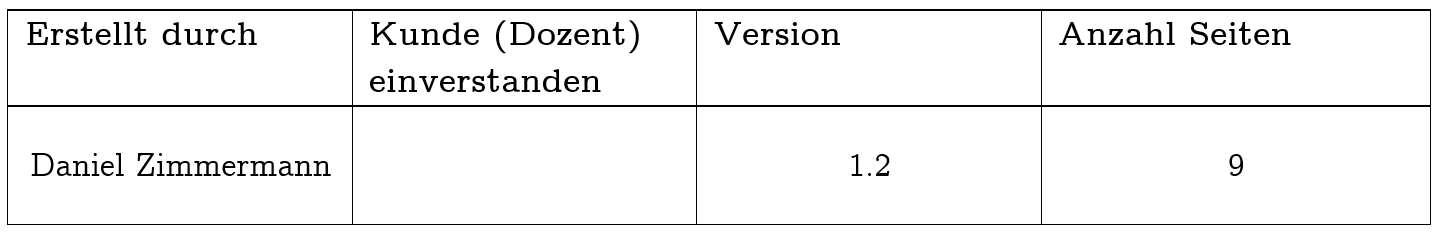
\includegraphics[width=1 \textwidth]{bilder/Pflichtenheft_6.PNG}
